\begin{figure}[H]
\centering
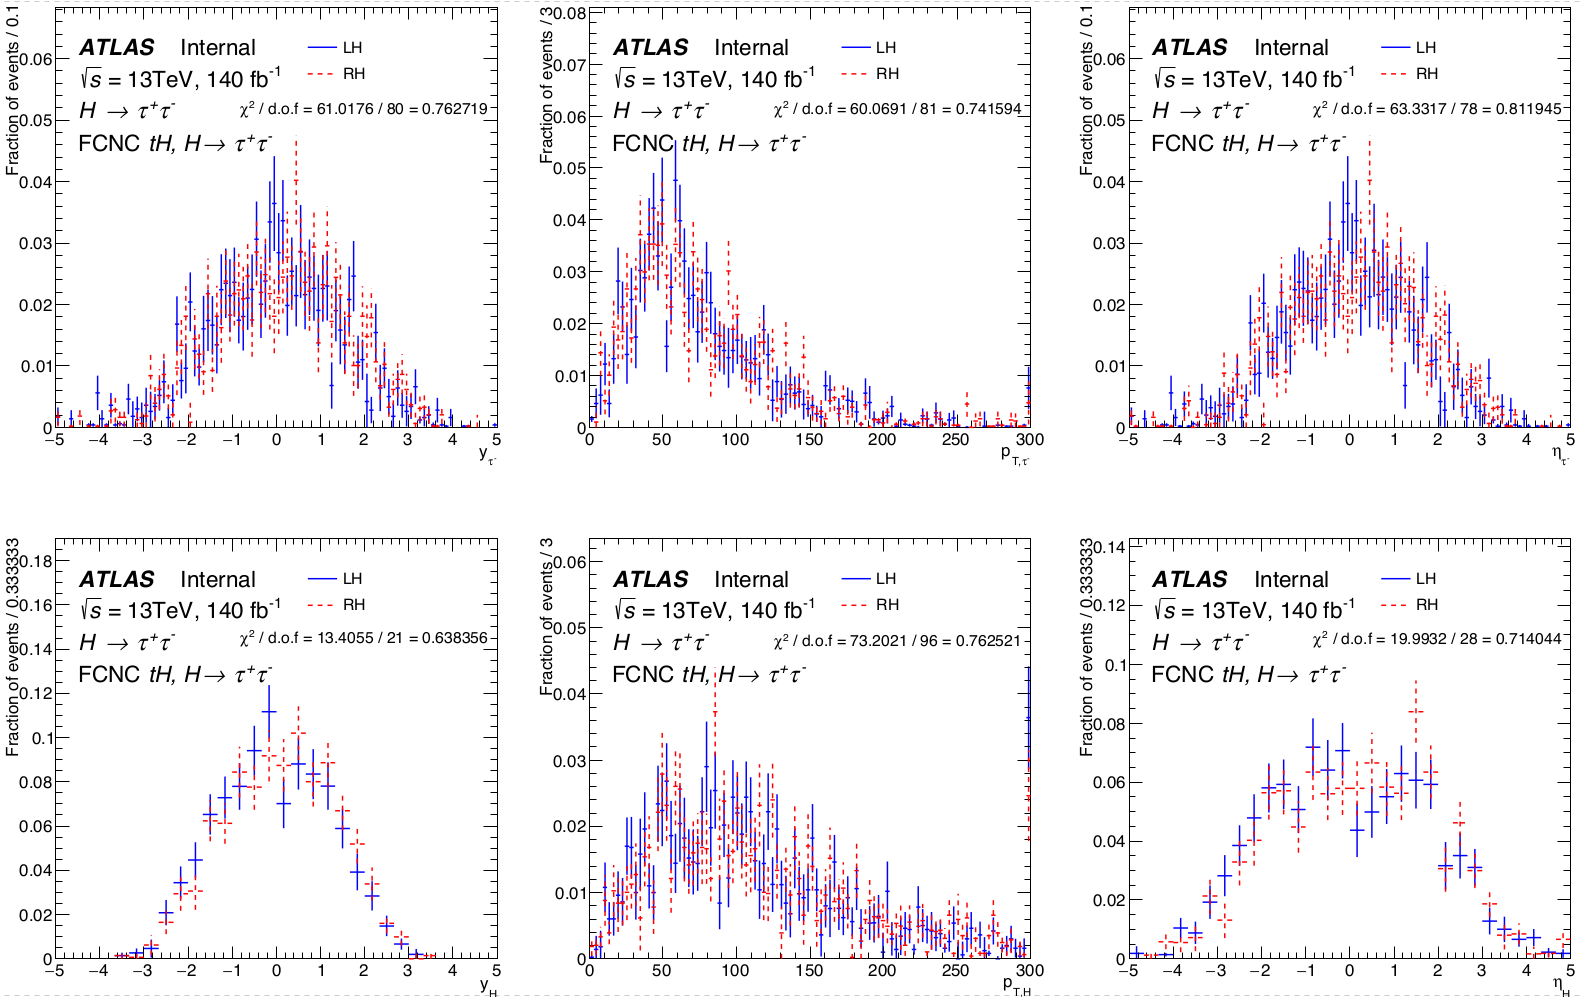
\includegraphics[width=\textwidth]{\FCNCFigures/screenshot/LHRHTruth.png}
\caption{六维左手算符(LH)和右手算符(RH)所引发的FCNC信号比较,当$\chi^2/\mathrm{d.o.f}>2$时表明约有95\%的置信度排除两个直方图一样的假设,这里$\chi^2/\mathrm{d.o.f}$都小于1说明,二者没有明显区别。}
\label{fig:LHRHTruth}
\end{figure}